% ICT 4442 Deep Learning Mini Project -- Phase 3 Final Report (Part C)
% Build: pdflatex final_report && pdflatex final_report
\documentclass[conference,onecolumn,a4paper,10pt]{IEEEtran}

\usepackage[a4paper,left=19mm,right=19mm,top=18mm,bottom=18mm]{geometry}
\usepackage[T1]{fontenc}
\usepackage{newtxtext,newtxmath}
\renewcommand{\ttdefault}{pcr}
\usepackage{amsmath}
\usepackage{graphicx}
\usepackage{booktabs}
\usepackage{array}
\usepackage{tabularx}
\usepackage[table]{xcolor}
\usepackage{tikz}
\usetikzlibrary{arrows.meta,positioning}
\usepackage{url}
\usepackage[hidelinks]{hyperref}

\graphicspath{{figures/}}
\pagestyle{empty}
\setlength{\emergencystretch}{1.5em}
\renewcommand{\IEEEkeywordsname}{Keywords}
\newcolumntype{L}[1]{>{\raggedright\arraybackslash}p{#1}}
\newcolumntype{Y}{>{\raggedright\arraybackslash}X}

% model colours (same as the figures)
\definecolor{mMLP}{HTML}{4C72B0}
\definecolor{mCNN}{HTML}{DD8452}
\definecolor{mLSTM}{HTML}{55A868}
\definecolor{mBERT}{HTML}{C44E52}
\definecolor{mGray}{HTML}{6A6A6A}

\begin{document}

%================================================================ COVER
\begin{titlepage}
\centering
\vspace*{6mm}
{\fontsize{16}{22}\selectfont\bfseries
COMPARATIVE ANALYSIS OF DEEP LEARNING\\
ARCHITECTURES FOR SENTIMENT ANALYSIS\\
OF MOVIE REVIEWS\par}
\vspace{12mm}
{\fontsize{14}{19}\selectfont\bfseries
Final report on\\
Deep Learning Project\\
{[}ICT-4442{]}\par}
\vspace{14mm}
{\fontsize{14}{19}\selectfont Submitted By\par}
\vspace{6mm}
{\fontsize{14}{20}\selectfont\bfseries
Meesha Gupta (230953090)\\
Ratul Jha (230953338)\\
Harshavardhan Reddy (230953396)\\
Kshitij Singh (230953460)\par}
\vspace{12mm}

\includegraphics[width=0.30\linewidth]{mit_logo.png}\par
\vspace{14mm}
{\fontsize{14}{19}\selectfont\bfseries
SCHOOL OF COMPUTER ENGINEERING\\
MANIPAL INSTITUTE OF TECHNOLOGY,\\
MANIPAL ACADEMY OF HIGHER EDUCATION\par}
\vspace{12mm}
{\fontsize{14}{19}\selectfont\bfseries OCTOBER 2026\par}
\end{titlepage}

%================================================================ TITLE
\title{Comparative Analysis of Deep Learning\\ Architectures for Sentiment Analysis\\ of Movie Reviews}

\author{\IEEEauthorblockN{Meesha Gupta (230953090),\quad Ratul Jha (230953338),\\
Harshavardhan Reddy (230953396),\quad Kshitij Singh (230953460)}
\IEEEauthorblockA{School of Computer Engineering, Manipal Institute of Technology\\
Manipal Academy of Higher Education, Manipal, India\\
{\fontsize{9}{11}\selectfont\upshape\ttfamily Code: https://github.com/HarshavardhanReddy585/imdb-sentiment-analysis-ict4442}}}

\maketitle
\thispagestyle{empty}

\begin{abstract}
Deciding whether a movie review is positive or negative requires a model to weigh word choice, negation and contrast across long, informal text. We compare four deep-learning architecture families on this task using the IMDb Large Movie Review Dataset, under one shared protocol: a 20,000/5,000 train/validation split of the official training set, a single evaluation on the untouched 25,000-review test set, and the same decision threshold and metrics for every model. The models are a multi-layer perceptron (MLP) over averaged word embeddings, a one-dimensional convolutional network (1D-CNN) with 3-, 4- and 5-word filters, a bidirectional LSTM (BiLSTM), and the pretrained Transformer DistilBERT fine-tuned end to end. DistilBERT is the most accurate model, with 90.83\% test accuracy, an F1-score of 0.907 and a ROC-AUC of 0.970. Among the models trained from scratch, the order-free MLP (88.56\%) significantly outperforms the 1D-CNN (87.32\%) and the BiLSTM (87.22\%) by McNemar's test, while training in a fraction of their time. Error analysis shows that DistilBERT's advantage is concentrated in reviews shorter than 300 words and reverses on very long reviews because of its 256-token input limit, and that reviews containing contrastive wording are the hardest case for every model. Pretraining therefore gives a clear but costly improvement, and a well-regularised bag-of-embeddings model remains a strong, inexpensive baseline.
\end{abstract}

\begin{IEEEkeywords}
Sentiment analysis, IMDb movie reviews, text classification, multi-layer perceptron, convolutional neural network, bidirectional LSTM, DistilBERT, transfer learning.
\end{IEEEkeywords}

%================================================================ I
\section{Introduction}
Online movie reviews are one of the largest public sources of opinionated text, and labelling a review as positive or negative automatically is useful for recommendation, audience analytics and content moderation. Sentiment in long reviews is not always carried by isolated words. Reviewers negate opinions (``not as bad as I expected''), change their stance halfway through (``the first hour is dull, but the ending is superb''), and spend most of a review retelling the plot before giving a one-line verdict. A model therefore has to decide how much of the surrounding context it needs, which makes the task a natural test bed for comparing neural architectures.

The IMDb Large Movie Review Dataset~\cite{maas2011} is the standard benchmark for this problem. Its two classes are balanced, its official train/test split is fixed, and its reviews are long enough (a median of 175 words) for word order and long-range context to matter.

This project compares four architecture families on exactly the same binary task, one owned by each team member: an MLP over averaged word embeddings that ignores word order, a 1D-CNN that detects local phrases, a BiLSTM that reads the whole review in both directions, and the pretrained Transformer DistilBERT~\cite{sanh2019}. All four use the same split, the same threshold and the same metrics, so that differences in the results can be attributed to the architectures themselves. The scope is limited to binary, document-level, English sentiment classification.

The report is organised as follows. Section~II reviews related work and Section~III states the objectives. Section~IV describes each model, and Section~V gives the shared experimental protocol. Section~VI presents and explains the results, including a statistical comparison and an error analysis. Sections~VII and~VIII conclude and outline future work.

%================================================================ II
\section{Literature Review}

\subsection{The IMDb Benchmark and Word Representations}
Maas et al.~\cite{maas2011} released the 50,000-review IMDb corpus used here and showed that word vectors learned together with a sentiment signal outperform purely unsupervised vectors on this task. Distributed representations such as Word2Vec~\cite{mikolov2013} and GloVe~\cite{pennington2014} showed that dense embeddings capture lexical similarity, which motivates the learned 128-dimensional embedding layer shared by our three scratch-trained models. These static vectors give a word the same meaning in every context, and averaging them, as our MLP does, also discards word order entirely.

\subsection{Convolutional Models}
Kim~\cite{kim2014} showed that a single convolutional layer with several filter widths followed by max-over-time pooling is a strong sentence classifier, because each filter behaves like a learned n-gram detector. Zhang and Wallace~\cite{zhang2017} studied the sensitivity of such networks to filter widths, number of feature maps and dropout, and recommended widths around 3--5 and moderate dropout; our 1D-CNN follows this guidance. Compared with the MLP, a CNN sees local word order, but max pooling keeps only the strongest response of each filter and loses where in the review it occurred.

\subsection{Recurrent Models}
Hochreiter and Schmidhuber~\cite{hochreiter1997} introduced the LSTM, whose input, forget and output gates mitigate vanishing gradients and allow information to persist across long sequences. Schuster and Paliwal~\cite{schuster1997} proposed bidirectional recurrent networks, which read a sequence in both directions so that every position is informed by both past and future context. Our BiLSTM combines both ideas. In principle it can model negation scope and long-range contrast, but it is sequential, slower to train, and must compress a whole review into a fixed-size state.

\subsection{Attention, Pretraining and Transfer Learning}
Vaswani et al.~\cite{vaswani2017} replaced recurrence with self-attention, letting every token attend directly to every other token. ELMo~\cite{peters2018} and ULMFiT~\cite{howard2018} showed that representations pretrained on large corpora and then fine-tuned transfer well to text classification, including IMDb. BERT~\cite{devlin2019} combined both ideas with bidirectional masked-language-model pretraining. Sanh et al.~\cite{sanh2019} distilled BERT into DistilBERT, which keeps about 97\% of BERT's language-understanding performance with 40\% fewer parameters. Sun et al.~\cite{sun2019} studied how to fine-tune BERT for text classification and report accuracies above 94\% on IMDb, and found that keeping both the beginning and the end of long reviews works better than keeping only the beginning.

\subsection{The Gap Addressed by This Work}
Most of these papers report a single architecture under their own preprocessing, split and tuning budget, so their numbers cannot be compared directly. This project trains one representative of each family under one protocol, evaluates all of them once on the same test set, tests whether the differences are statistically significant, and analyses where each model fails. Table~\ref{tab:lit} summarises how the core papers relate to the four models.

\begin{table}[!t]
\caption{Summary of the core literature and its relation to this project}\label{tab:lit}
\centering\footnotesize\renewcommand{\arraystretch}{1.15}
\begin{tabularx}{\linewidth}{@{}L{3.0cm}L{3.1cm}L{2.2cm}YL{1.9cm}@{}}
\toprule
\textbf{Paper} & \textbf{Method} & \textbf{Dataset} & \textbf{Key result} & \textbf{Used by} \\
\midrule
Maas et al. 2011~\cite{maas2011} & Sentiment-aware word vectors & IMDb 50k & Introduced the benchmark; supervised vectors beat unsupervised ones & All \\
Mikolov et al. 2013~\cite{mikolov2013} & Word2Vec embeddings & Large corpora & Dense vectors capture lexical regularities & MLP, CNN, BiLSTM \\
Kim 2014~\cite{kim2014} & CNN, widths 3/4/5, max pooling & Sentence benchmarks & A simple CNN is competitive with deeper models & 1D-CNN \\
Zhang \& Wallace 2017~\cite{zhang2017} & CNN sensitivity analysis & Sentence benchmarks & Practical ranges for widths, filters and dropout & 1D-CNN \\
Hochreiter \& Schmidhuber 1997~\cite{hochreiter1997} & LSTM gating & Synthetic sequences & Learns dependencies over long time lags & BiLSTM \\
Schuster \& Paliwal 1997~\cite{schuster1997} & Bidirectional RNN & Speech (TIMIT) & Two-direction context improves sequence modelling & BiLSTM \\
Vaswani et al. 2017~\cite{vaswani2017} & Self-attention Transformer & WMT translation & Attention alone outperforms recurrent models & DistilBERT \\
Howard \& Ruder 2018~\cite{howard2018} & ULMFiT fine-tuning & IMDb and 5 others & Pretrain-then-fine-tune sharply cuts IMDb error & DistilBERT \\
Devlin et al. 2019~\cite{devlin2019} & BERT masked-LM pretraining & GLUE, SQuAD & State of the art on 11 tasks & DistilBERT \\
Sanh et al. 2019~\cite{sanh2019} & Distillation of BERT & GLUE, IMDb & 40\% smaller, 60\% faster, about 97\% of BERT & DistilBERT \\
\bottomrule
\end{tabularx}
\end{table}

%================================================================ III
\section{Objectives}
\begin{enumerate}
\item To implement four architecture families (MLP, 1D-CNN, BiLSTM and DistilBERT) for binary sentiment classification on IMDb under one common preprocessing and evaluation protocol.
\item To compare the four models on the untouched 25,000-review test set using accuracy, precision, recall, F1-score and ROC-AUC, together with parameter count and training cost, and to explain the observed differences in terms of architecture.
\item To analyse misclassified reviews (by length, contrastive wording and model agreement) to identify which kinds of review each model handles poorly.
\end{enumerate}

%================================================================ IV
\section{Methodology}
Fig.~\ref{fig:overview} shows the four pipelines. The MLP, 1D-CNN and BiLSTM share the same word-level tokenizer and an embedding layer of the same shape, trained from scratch, and differ only in the encoder that turns the sequence of word vectors into a fixed-length review vector. DistilBERT uses its own pretrained WordPiece tokenizer and Transformer encoder. Every model ends in a single output unit $z$ and is trained with the binary cross-entropy loss on $\hat{y}=\sigma(z)$:
\begin{equation}
\mathcal{L} = -\frac{1}{N}\sum_{i=1}^{N}\big[y_i\log\hat{y}_i + (1-y_i)\log(1-\hat{y}_i)\big],
\end{equation}
to which the scratch models add an L2 penalty of $10^{-4}\lVert W\rVert^2$ on the weights $W$ of their hidden dense layer. A review is labelled positive when $\hat{y}\ge 0.5$. Table~\ref{tab:config} lists every hyperparameter side by side; the values were chosen on the validation set in Phase~2 and then frozen.

\begin{figure}[!t]
\centering
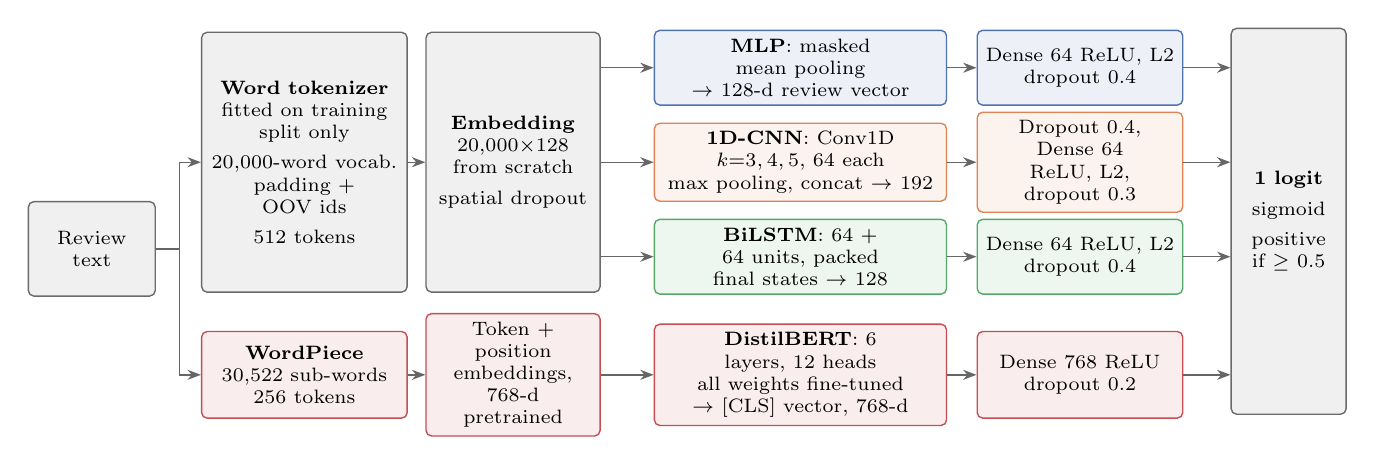
\begin{tikzpicture}[font=\scriptsize,
  blk/.style={draw=#1, fill=#1!10, rounded corners=2pt, align=center, inner sep=3pt, line width=0.5pt},
  to/.style={-{Stealth[length=1.7mm]}, line width=0.5pt, draw=black!60}]
\node[blk=mGray, text width=1.4cm, minimum height=1.2cm] (rev) at (0,0) {Review\\text};
\node[blk=mGray, text width=2.4cm, minimum height=3.3cm] (tok) at (2.7,1.1)
  {\textbf{Word tokenizer}\\fitted on training\\split only\\[3pt]20,000-word vocab.\\padding + OOV ids\\[3pt]512 tokens};
\node[blk=mGray, text width=2.0cm, minimum height=3.3cm] (emb) at (5.35,1.1)
  {\textbf{Embedding}\\20,000$\times$128\\from scratch\\[3pt]spatial dropout};
\node[blk=mBERT, text width=2.4cm, minimum height=1.1cm] (wp) at (2.7,-1.6)
  {\textbf{WordPiece}\\30,522 sub-words\\256 tokens};
\node[blk=mBERT, text width=2.0cm, minimum height=1.1cm] (pe) at (5.35,-1.6)
  {Token + position\\embeddings, 768-d\\pretrained};
\node[blk=mMLP, text width=3.5cm, minimum height=0.95cm] (m1) at (9.0,2.3)
  {\textbf{MLP}: masked mean pooling\\$\rightarrow$ 128-d review vector};
\node[blk=mCNN, text width=3.5cm, minimum height=0.95cm] (m2) at (9.0,1.1)
  {\textbf{1D-CNN}: Conv1D $k{=}3,4,5$, 64 each\\max pooling, concat $\rightarrow$ 192};
\node[blk=mLSTM, text width=3.5cm, minimum height=0.95cm] (m3) at (9.0,-0.1)
  {\textbf{BiLSTM}: 64 + 64 units, packed\\final states $\rightarrow$ 128};
\node[blk=mBERT, text width=3.5cm, minimum height=1.1cm] (m4) at (9.0,-1.6)
  {\textbf{DistilBERT}: 6 layers, 12 heads\\all weights fine-tuned\\$\rightarrow$ [CLS] vector, 768-d};
\node[blk=mMLP, text width=2.4cm, minimum height=0.95cm] (h1) at (12.55,2.3) {Dense 64 ReLU, L2\\dropout 0.4};
\node[blk=mCNN, text width=2.4cm, minimum height=0.95cm] (h2) at (12.55,1.1) {Dropout 0.4, Dense 64\\ReLU, L2, dropout 0.3};
\node[blk=mLSTM, text width=2.4cm, minimum height=0.95cm] (h3) at (12.55,-0.1) {Dense 64 ReLU, L2\\dropout 0.4};
\node[blk=mBERT, text width=2.4cm, minimum height=1.1cm] (h4) at (12.55,-1.6) {Dense 768 ReLU\\dropout 0.2};
\node[blk=mGray, text width=1.25cm, minimum height=4.9cm] (out) at (15.2,0.35) {\textbf{1 logit}\\[3pt]sigmoid\\[3pt]positive\\if $\ge$ 0.5};
\draw[to] (rev.east) -- ++(0.3,0) |- (tok.west);
\draw[to] (rev.east) -- ++(0.3,0) |- (wp.west);
\draw[to] (tok) -- (emb);
\draw[to] (wp) -- (pe);
\foreach \m in {m1,m2,m3} {\draw[to] (emb.east |- \m.west) -- (\m.west);}
\draw[to] (pe) -- (m4);
\foreach \m/\h in {m1/h1,m2/h2,m3/h3,m4/h4} {\draw[to] (\m) -- (\h);}
\foreach \h in {h1,h2,h3,h4} {\draw[to] (\h.east) -- (\h.east -| out.west);}
\end{tikzpicture}
\caption{The four models. The scratch models share the tokenizer and the shape of the embedding layer (each trains its own copy) and differ in the encoder; DistilBERT uses its own pretrained tokenizer and encoder. All four end in a single logit and a 0.5 threshold.}
\label{fig:overview}
\end{figure}

\begin{table}[!t]
\caption{Model and training configuration}\label{tab:config}
\centering\footnotesize\renewcommand{\arraystretch}{1.15}
\begin{tabularx}{\linewidth}{@{}L{2.9cm}YYYY@{}}
\toprule
 & \textbf{\color{mMLP}MLP} & \textbf{\color{mCNN}1D-CNN} & \textbf{\color{mLSTM}BiLSTM} & \textbf{\color{mBERT}DistilBERT} \\
\midrule
Input & 512 word tokens & 512 word tokens & 512 word tokens & 256 WordPiece tokens \\
Embedding & 20,000$\times$128, scratch & 20,000$\times$128, scratch & 20,000$\times$128, scratch & 768-d, pretrained \\
Input dropout & spatial 0.2 & spatial 0.3 & spatial 0.3 + 0.3 & -- \\
Encoder & masked mean & Conv1D 3/4/5$\times$64, max pool & BiLSTM 64+64, packed & 6 Transformer layers \\
Head & Dense 64, dropout 0.4 & Dense 64, dropout 0.4/0.3 & Dense 64, dropout 0.4 & Dense 768, dropout 0.2 \\
Parameters & 2,568,321 & 2,670,913 & 2,667,649 & 66,954,241 \\
Optimiser & Adam~\cite{kingma2015} & Adam & Adam & AdamW~\cite{loshchilov2019}, decay 0.01 \\
Learning rate & $10^{-3}$ & $10^{-3}$ & $5\times10^{-4}$ & $2\times10^{-5}$ \\
LR schedule & halve on plateau & halve on plateau & halve on plateau & 10\% warm-up, linear decay \\
Batch size & 64 & 512 & 64 & 16 \\
Max epochs / patience & 20 / 3 & 12 / 2 & 20 / 3 & 5 / 2 \\
Other & L2 $10^{-4}$ & L2 $10^{-4}$ & L2 $10^{-4}$ & clip norm 1.0, fp16 \\
\bottomrule
\end{tabularx}
\end{table}

\subsection{Multi-Layer Perceptron Baseline (Owner: Kshitij Singh)}
\textit{Architecture.} Embedding (20,000$\times$128) $\rightarrow$ spatial dropout 0.2 $\rightarrow$ mean pooling over the non-padding tokens $\rightarrow$ dense layer of 64 ReLU units with L2 penalty $10^{-4}$ $\rightarrow$ dropout 0.4 $\rightarrow$ one output unit. Spatial dropout, a variant of dropout~\cite{srivastava2014}, removes whole embedding dimensions for a review rather than individual values. This regularises the 2.56\,M-parameter embedding table, which accounts for almost all of the model's 2,568,321 parameters.

\textit{Training.} Adam with learning rate $10^{-3}$, batch size 64, at most 20 epochs, the learning rate halved after an epoch without improvement in validation loss, and early stopping with patience~3.

\textit{Justification.} Averaging embeddings turns a review into an order-free ``bag of word vectors''. The MLP is the baseline that answers the question ``how far can we get from which words appear, ignoring their order?'', and every gain made by the other models is measured against it. Fig.~\ref{fig:cmlp} shows that its validation loss is lowest after only two epochs (0.266, validation accuracy 89.48\%), after which the model starts to memorise the training set.

\begin{figure}[!t]
\centering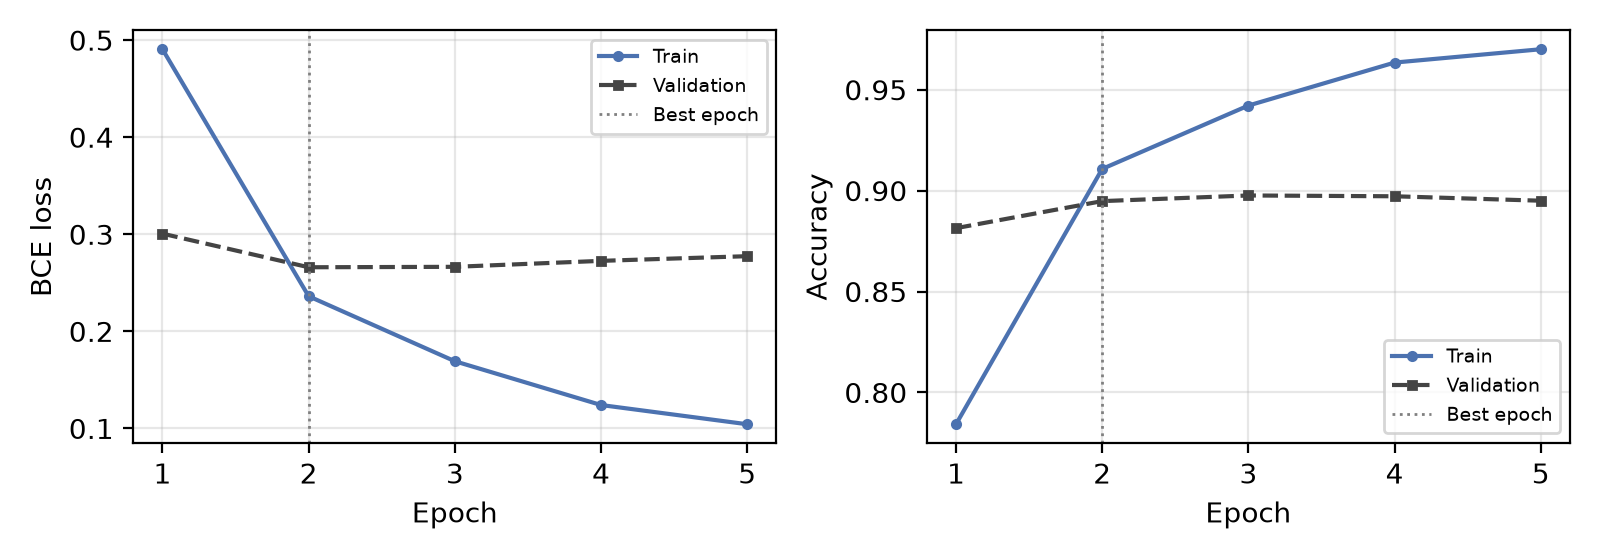
\includegraphics[width=0.82\linewidth]{curves_mlp.png}
\caption{MLP training and validation curves. Best epoch 2 of 5 (validation loss 0.266, validation accuracy 89.48\%).}\label{fig:cmlp}
\end{figure}

\subsection{One-Dimensional CNN (Owner: Ratul Jha)}
\textit{Architecture.} Embedding (20,000$\times$128) $\rightarrow$ spatial dropout 0.3 $\rightarrow$ three parallel 1D convolutions with 64 filters each and kernel widths 3, 4 and 5 (ReLU) $\rightarrow$ global max pooling over time for each branch $\rightarrow$ concatenation (192 features) $\rightarrow$ dropout 0.4 $\rightarrow$ dense 64 ReLU (L2 $10^{-4}$) $\rightarrow$ dropout 0.3 $\rightarrow$ one output unit; 2,670,913 parameters in total.

\textit{Training.} Adam with learning rate $10^{-3}$, batch size 512, at most 12 epochs, the same learning-rate schedule as the MLP, and early stopping with patience~2.

\textit{Justification.} Following Kim~\cite{kim2014} and Zhang and Wallace~\cite{zhang2017}, each filter acts as a trainable detector for 3- to 5-word phrases such as ``not worth watching'' or ``one of the best'', and max pooling keeps each phrase's strongest occurrence wherever it appears. This adds local word order to the MLP baseline while remaining fully parallel. The large batch makes each epoch fast but gives fewer updates per epoch, so the CNN needs five epochs to reach its best validation loss (0.309, Fig.~\ref{fig:ccnn}).

\begin{figure}[!t]
\centering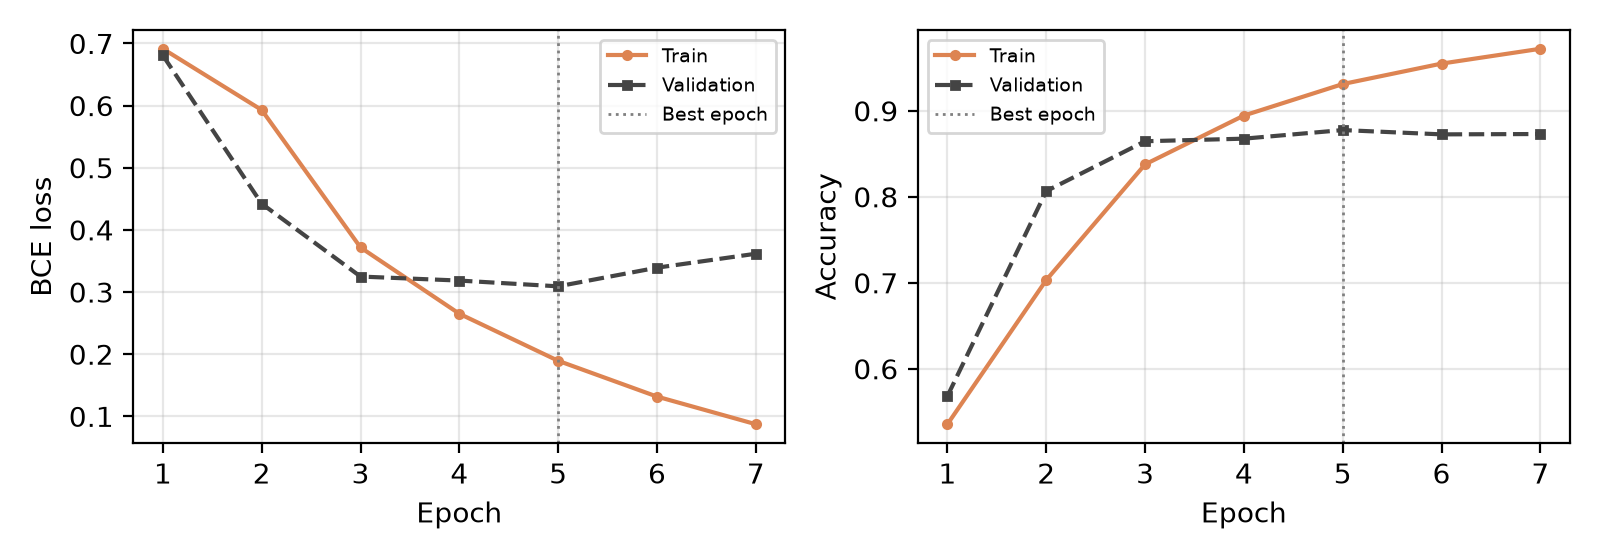
\includegraphics[width=0.82\linewidth]{curves_cnn.png}
\caption{1D-CNN training and validation curves. Best epoch 5 of 7 (validation loss 0.309, validation accuracy 87.76\%).}\label{fig:ccnn}
\end{figure}

\subsection{Bidirectional LSTM (Owner: Harshavardhan Reddy)}
\textit{Architecture.} Embedding (20,000$\times$128) $\rightarrow$ spatial dropout 0.3 $\rightarrow$ input dropout 0.3 $\rightarrow$ bidirectional LSTM with 64 units per direction $\rightarrow$ concatenation of the final forward and backward hidden states (128) $\rightarrow$ dense 64 ReLU (L2 $10^{-4}$) $\rightarrow$ dropout 0.4 $\rightarrow$ one output unit; 2,667,649 parameters. The padded sequences are packed, so the forward LSTM stops at the last real word and the backward LSTM starts there; padding never enters the recurrent state.

\textit{Training.} Adam with learning rate $5\times10^{-4}$ (half that of the other scratch models, the value selected in Phase~2), batch size 64, at most 20 epochs, the same learning-rate schedule, and early stopping with patience~3.

\textit{Justification.} The LSTM's gates~\cite{hochreiter1997} let it carry information across the whole review, and reading in both directions~\cite{schuster1997} lets the review representation depend on both its opening and its conclusion. It is the only scratch model that can, in principle, model negation scope and ``\ldots but'' contrasts across a sentence boundary. Fig.~\ref{fig:clstm} shows that it reaches its best validation loss (0.293) at epoch~3, after which training accuracy keeps rising to 98\% while validation loss climbs.

\begin{figure}[!t]
\centering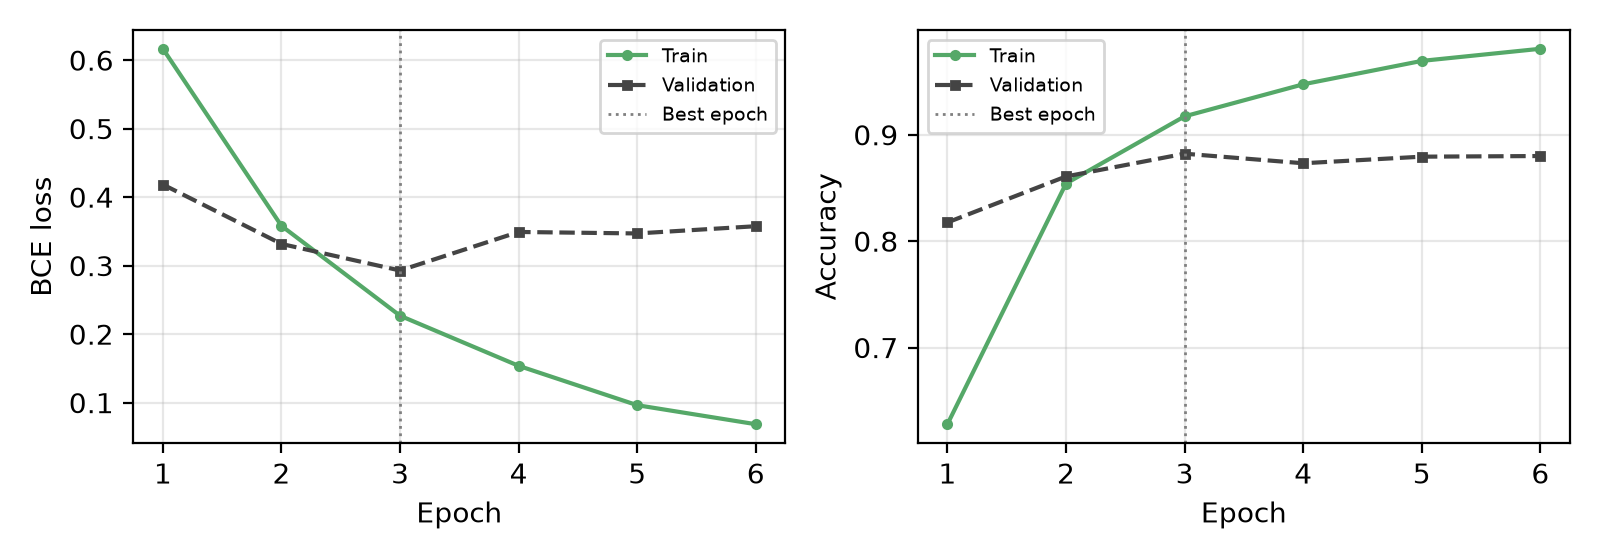
\includegraphics[width=0.82\linewidth]{curves_bilstm.png}
\caption{BiLSTM training and validation curves. Best epoch 3 of 6 (validation loss 0.293, validation accuracy 88.22\%).}\label{fig:clstm}
\end{figure}

\subsection{DistilBERT (Owner: Meesha Gupta)}
\textit{Architecture.} The pretrained \texttt{distilbert-base-uncased} model~\cite{sanh2019}: six Transformer encoder layers with 12 attention heads, hidden size 768 and a 30,522-entry WordPiece vocabulary, followed by a 768-unit pre-classifier dense layer with ReLU and dropout 0.2 and a single-logit output on the \texttt{[CLS]} token. All 66,954,241 parameters are fine-tuned.

\textit{Training.} AdamW~\cite{loshchilov2019} with learning rate $2\times10^{-5}$ and weight decay 0.01, linear warm-up over the first 10\% of steps followed by linear decay, gradient-norm clipping at 1.0, batch size 16, at most 5 epochs, early stopping with patience~2, and mixed precision (fp16). Inputs are truncated to 256 WordPiece tokens so that training fits in the 8\,GB of GPU memory available.

\textit{Justification.} DistilBERT represents the attention-based, pretrain-then-fine-tune family that defines the current state of the art~\cite{devlin2019,sun2019}, at a size that can be fine-tuned on a laptop GPU. Its self-attention gives every token direct access to every other token, and its pretraining provides knowledge of English that the scratch models must learn from 20,000 reviews alone. Fig.~\ref{fig:cbert} shows that it overfits fastest of all: its validation loss is lowest at epoch~2 (0.295) and rises to 0.446 by epoch~4 while training accuracy reaches 98.4\%.

\begin{figure}[!t]
\centering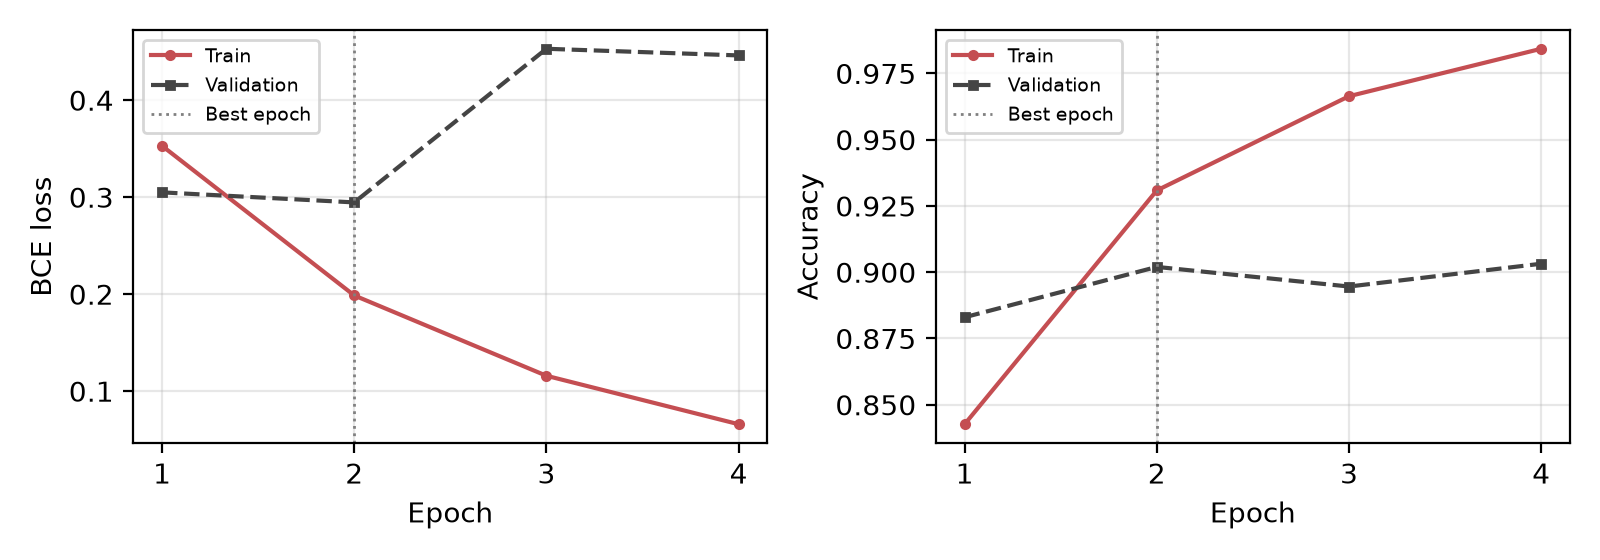
\includegraphics[width=0.82\linewidth]{curves_distilbert.png}
\caption{DistilBERT training and validation curves. Best epoch 2 of 4 (validation loss 0.295, validation accuracy 90.20\%).}\label{fig:cbert}
\end{figure}

%================================================================ V
\section{Experimental Setup}

\subsection{Dataset}
The IMDb Large Movie Review Dataset~\cite{maas2011} contains 50,000 highly polar English reviews (at most 30 per film), evenly split into 25,000 training and 25,000 test reviews, each with 12,500 positive and 12,500 negative examples. Reviews with a rating of at most 4/10 are labelled negative and reviews rated at least 7/10 positive, so neutral reviews are excluded. The median training review is 175 words long, and 92.5\% of training reviews fit within 512 words (Fig.~\ref{fig:len}).

\begin{figure}[!t]
\centering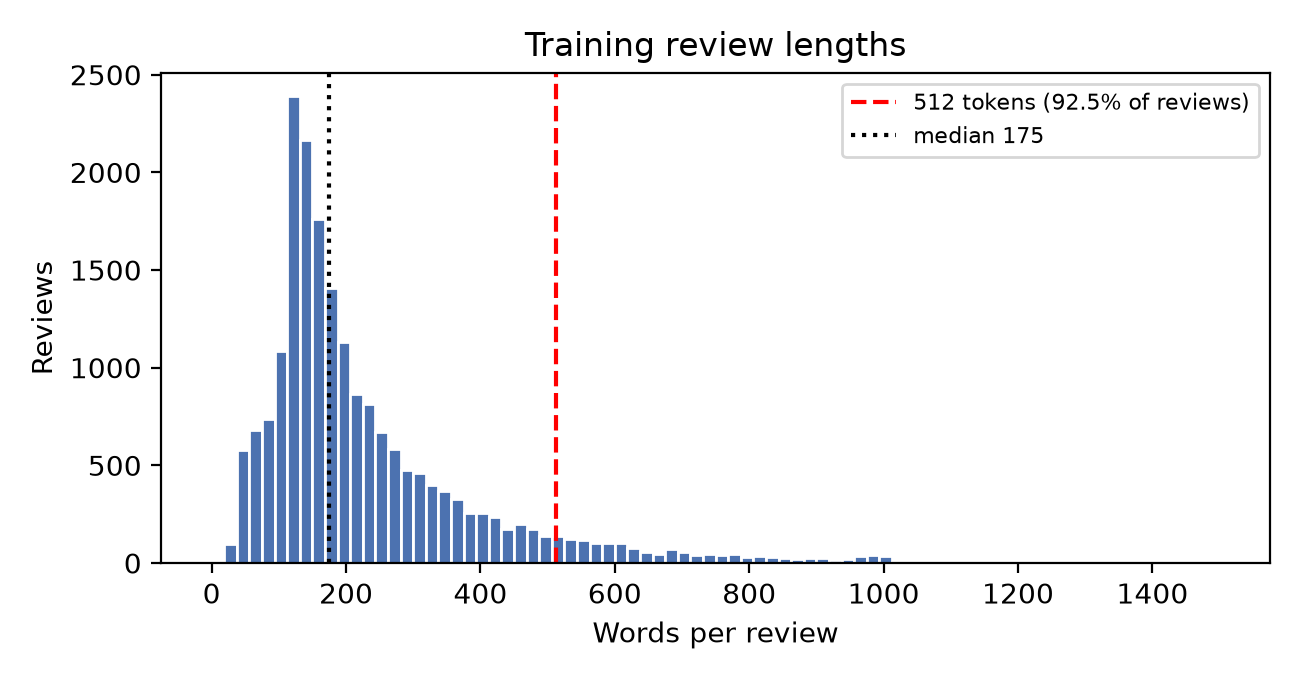
\includegraphics[width=0.66\linewidth]{review_length_distribution.png}
\caption{Distribution of review lengths in the 20,000-review training split. The dashed line marks the 512-token limit used by the scratch models.}\label{fig:len}
\end{figure}

\subsection{Train, Validation and Test Split}
The official training set is split, stratified by label with random seed 42, into 20,000 training and 5,000 validation reviews (Table~\ref{tab:split}). The validation set drives early stopping and the learning-rate schedule. The official 25,000-review test set is used only once, after training and model selection are complete.

\begin{table}[!t]
\caption{Data split shared by all four models}\label{tab:split}
\centering\footnotesize\renewcommand{\arraystretch}{1.15}
\begin{tabular}{@{}l l r r r l@{}}
\toprule
\textbf{Split} & \textbf{Source} & \textbf{Reviews} & \textbf{Positive} & \textbf{Negative} & \textbf{Used for} \\
\midrule
Train & official train set & 20,000 & 10,000 & 10,000 & weights, vocabulary \\
Validation & official train set & 5,000 & 2,500 & 2,500 & early stopping, LR schedule \\
Test & official test set & 25,000 & 12,500 & 12,500 & final evaluation only \\
\bottomrule
\end{tabular}
\end{table}

\subsection{Preprocessing}
For the scratch models, HTML line breaks are removed, text is lower-cased, punctuation is stripped and the text is split on whitespace. The vocabulary, fitted on the 20,000 training reviews only, keeps the 19,998 most frequent words plus a padding index and an out-of-vocabulary token. Sequences are post-padded or post-truncated to 512 tokens, which keeps the beginning of the longest reviews. DistilBERT must use its own pretrained WordPiece tokenizer, so its reviews are tokenised to 256 sub-word tokens. This is the only intended difference in input between the models, and it is a disadvantage for DistilBERT on long reviews.

\subsection{Training Protocol}
All models were implemented in PyTorch~\cite{paszke2019} (DistilBERT through the Hugging Face Transformers library~\cite{wolf2020}) and trained on a single NVIDIA GeForce RTX 3080 Laptop GPU (8\,GB) with random seed 42. After every epoch the model is scored on the validation set. The weights with the lowest validation loss are kept, and training stops when the validation loss has not improved for the patience given in Table~\ref{tab:config}. The test set therefore plays no part in model selection.

\subsection{Evaluation Metrics}
With TP, TN, FP and FN the true and false positives and negatives at threshold 0.5, we report
\begin{equation}
\text{Acc}=\frac{TP+TN}{N},\quad \text{P}=\frac{TP}{TP+FP},\quad \text{R}=\frac{TP}{TP+FN},\quad F_1=\frac{2\,\text{P}\,\text{R}}{\text{P}+\text{R}},
\end{equation}
together with the area under the ROC curve (ROC-AUC), which measures ranking quality independently of the threshold. To test whether two models differ by more than chance, we apply McNemar's test to their per-review correctness. With $b$ the number of test reviews only the first model gets right and $c$ the number only the second gets right,
\begin{equation}
\chi^2=\frac{(|b-c|-1)^2}{b+c},
\end{equation}
which follows a $\chi^2$ distribution with one degree of freedom under the hypothesis that both models have the same error rate. We also record the median time per training epoch and the time needed to score the full test set. All metrics, training histories and test-set probabilities are saved as files in the repository, and every table and figure in Section~VI is generated from them by a script.

%================================================================ VI
\section{Results and Discussion}

\subsection{Main Comparison}
Table~\ref{tab:results} reports the four models on the 25,000 test reviews, and Fig.~\ref{fig:roc} shows the same metrics graphically together with the ROC curves. DistilBERT is the best model on every metric, with 90.83\% accuracy, an F1-score of 0.9065 and a ROC-AUC of 0.9695. Among the models trained from scratch, the simplest one, the MLP, is the strongest (88.56\% accuracy, ROC-AUC 0.9531), ahead of the 1D-CNN (87.32\%) and the BiLSTM (87.22\%). The test results are within about one point of the validation results for every model, so the validation set was a reliable guide for model selection.

\begin{table}[!t]
\caption{Test-set comparison of the four models (25,000 reviews, threshold 0.5)}\label{tab:results}
\centering\footnotesize\renewcommand{\arraystretch}{1.15}
\begin{tabular}{@{}l r c c c c c c c r r@{}}
\toprule
\textbf{Model} & \textbf{Params} & \textbf{Acc.} & \textbf{Prec.} & \textbf{Recall} & \textbf{F1} & \textbf{ROC-AUC} & \textbf{Val acc.} & \textbf{Best ep.} & \textbf{s / epoch} & \textbf{Test inf. (s)} \\
\midrule
\color{mMLP}MLP        & 2.57\,M  & 0.8856 & 0.8957 & 0.8729 & 0.8842 & 0.9531 & 0.8948 & 2 & 2   & 0.25 \\
\color{mCNN}1D-CNN     & 2.67\,M  & 0.8732 & 0.8692 & 0.8787 & 0.8739 & 0.9446 & 0.8776 & 5 & 36  & 12.97 \\
\color{mLSTM}BiLSTM     & 2.67\,M  & 0.8722 & 0.8761 & 0.8670 & 0.8715 & 0.9436 & 0.8822 & 3 & 78  & 15.55 \\
\color{mBERT}DistilBERT & 66.95\,M & \textbf{0.9083} & \textbf{0.9248} & \textbf{0.8888} & \textbf{0.9065} & \textbf{0.9695} & \textbf{0.9020} & 2 & 108 & 57.14 \\
\bottomrule
\end{tabular}

\vspace{3pt}\parbox{\linewidth}{\scriptsize Precision, recall and F1 are for the positive class. ``s / epoch'' is the median epoch time and ``Test inf.'' the time to score all 25,000 test reviews. The laptop GPU's speed varied during the runs (for example, BiLSTM epochs took between 37 and 340\,s), so the timings are indicative and their ordering matters more than their exact values.}
\end{table}

\begin{figure}[!t]
\centering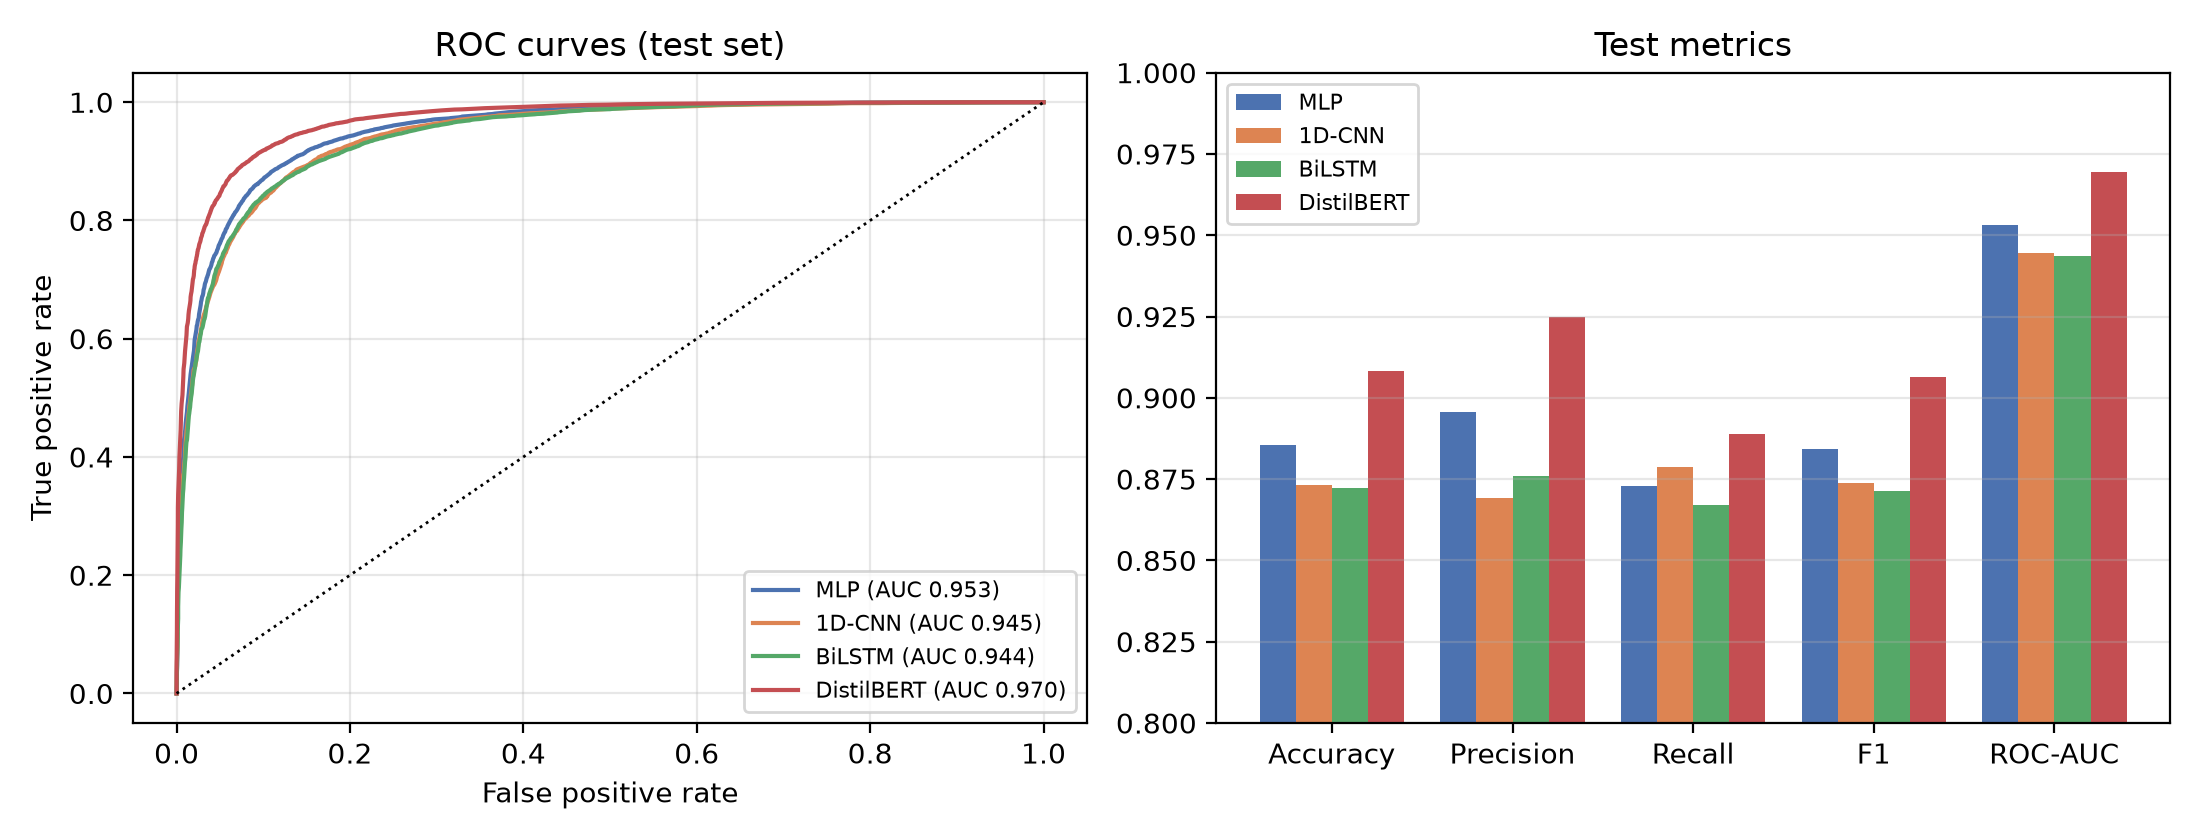
\includegraphics[width=\linewidth]{roc_and_metrics_test.png}
\caption{Left: ROC curves of the four models on the test set. Right: test accuracy, precision, recall, F1-score and ROC-AUC (the y-axis starts at 0.80).}\label{fig:roc}
\end{figure}

\subsection{Confusion Matrices and Statistical Significance}
Fig.~\ref{fig:cm} shows the confusion matrices. DistilBERT makes 2,293 errors, against 2,859 for the MLP, 3,169 for the 1D-CNN and 3,196 for the BiLSTM. Its advantage comes mainly from precision: it produces 903 false positives, against 1,270--1,653 for the scratch models, so it is much less often fooled into calling a negative review positive. The 1D-CNN is the only model with more false positives than false negatives, so it leans towards predicting the positive class.

Table~\ref{tab:mcnemar} gives McNemar's test for every pair of models. DistilBERT is significantly better than every scratch model ($p<10^{-24}$), and the MLP is significantly better than both the 1D-CNN and the BiLSTM. The 1D-CNN and the BiLSTM are statistically indistinguishable ($p=0.66$): each gets about 1,700 reviews right that the other gets wrong.

\begin{figure}[!t]
\centering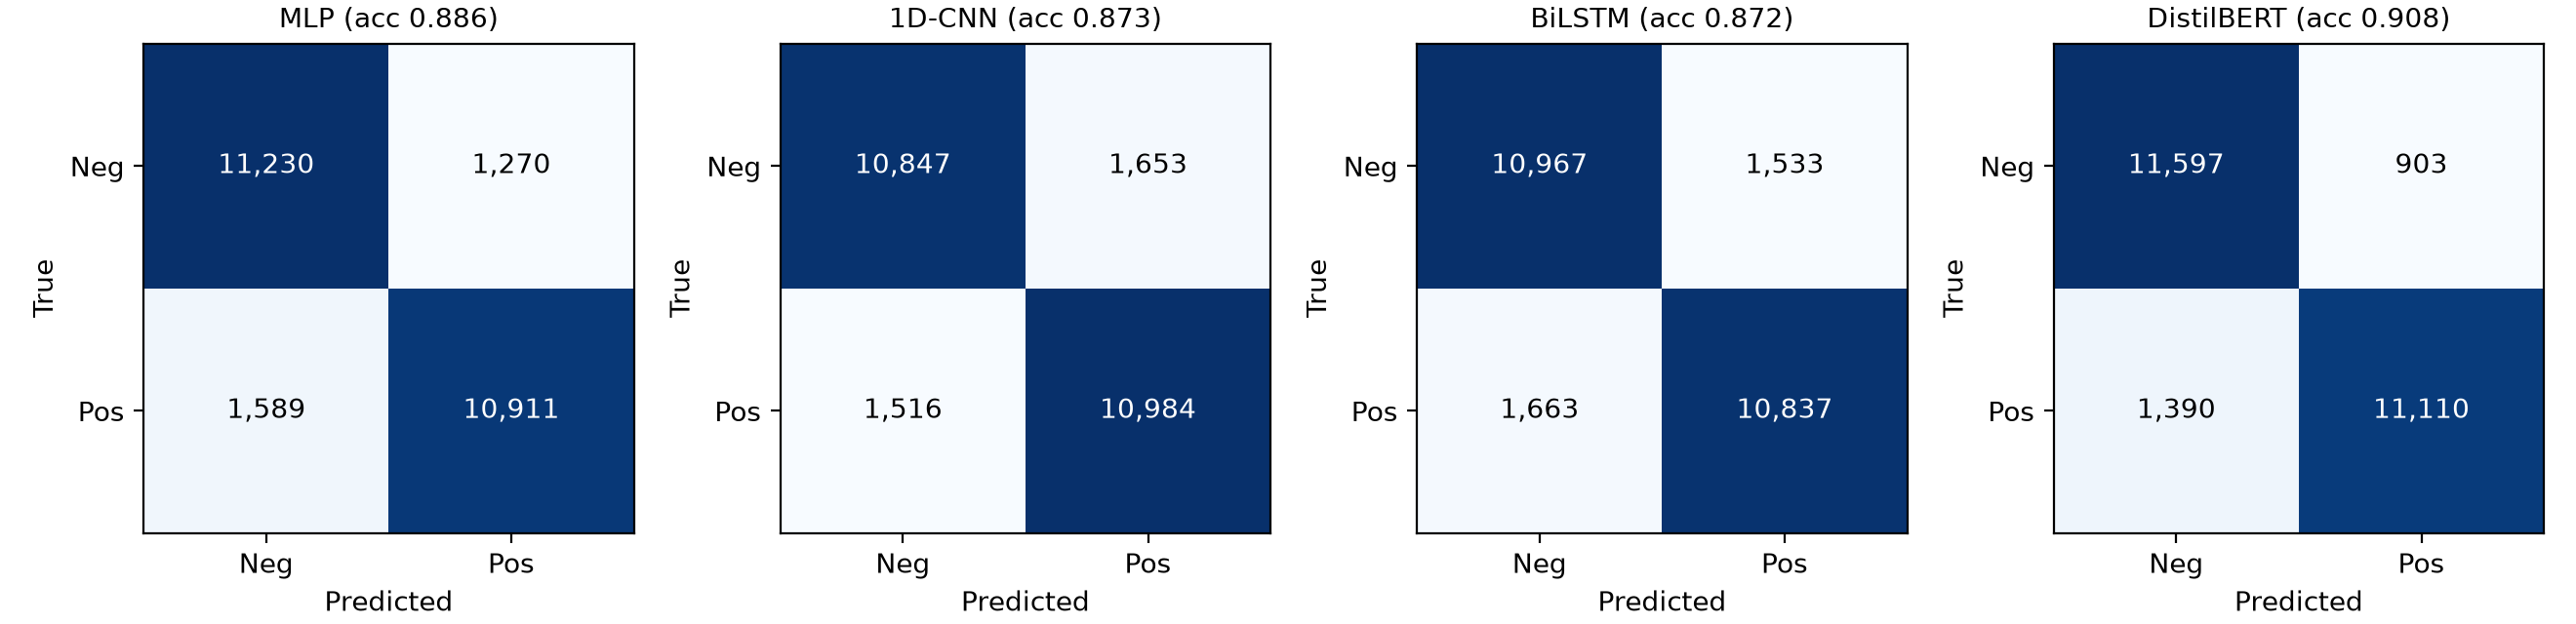
\includegraphics[width=\linewidth]{confusion_matrices_test.png}
\caption{Confusion matrices on the 25,000-review test set (rows: true class; columns: predicted class).}\label{fig:cm}
\end{figure}

\begin{table}[!t]
\caption{McNemar's test on per-review correctness (test set)}\label{tab:mcnemar}
\centering\footnotesize\renewcommand{\arraystretch}{1.15}
\begin{tabular}{@{}l r r r l@{}}
\toprule
\textbf{Model A vs. model B} & \textbf{Only A correct} & \textbf{Only B correct} & $\chi^2$ & \textbf{$p$-value} \\
\midrule
MLP vs. 1D-CNN & 1,663 & 1,353 & 31.7 & $1.8\times10^{-8}$ \\
MLP vs. BiLSTM & 1,239 & 902 & 52.7 & $3.8\times10^{-13}$ \\
1D-CNN vs. BiLSTM & 1,723 & 1,696 & 0.20 & 0.66 \\
MLP vs. DistilBERT & 1,213 & 1,779 & 106.7 & $5.2\times10^{-25}$ \\
1D-CNN vs. DistilBERT & 1,268 & 2,144 & 224.4 & $1.0\times10^{-50}$ \\
BiLSTM vs. DistilBERT & 1,303 & 2,206 & 231.9 & $2.3\times10^{-52}$ \\
\bottomrule
\end{tabular}
\end{table}

\subsection{Why the Models Perform Differently}
\textit{The pretrained Transformer wins.} Pretraining gives DistilBERT word meanings that depend on context and a knowledge of English syntax before it sees a single IMDb review, whereas the scratch models must learn everything, including their embeddings, from 20,000 labelled reviews. Our 90.8\% is below the more than 94\% that Sun et al.~\cite{sun2019} report for full BERT, which is consistent with the smaller distilled model and with the 256-token input limit discussed in Section~VI-D.

\textit{The bag-of-embeddings baseline beats the sequence models.} The MLP outperforming the 1D-CNN and the BiLSTM goes against the usual expectation, but it has a clear explanation. Sentiment in IMDb reviews is largely lexical: words such as ``worst'', ``waste'', ``superb'' and ``beautifully'' carry most of the signal, and a long review usually repeats its verdict several times. Averaging embeddings over the whole review uses every one of those cues and is hard to overfit. The CNN's max pooling instead keeps only the single strongest response of each filter, and the BiLSTM must squeeze a 500-word review into two 64-dimensional final states. The extra information these models can extract from word order therefore comes with more ways to fit noise, and with 20,000 training reviews the cost outweighs the gain: Figs.~\ref{fig:ccnn} and~\ref{fig:clstm} show both models reaching about 97--98\% training accuracy while their validation loss rises.

\textit{Cost of the improvement.} Moving from the MLP to DistilBERT gains 2.3 accuracy points and 1.6 ROC-AUC points, but it multiplies the parameter count by 26, the time per epoch by about 55 and the test inference time by more than 200, and it requires a GPU. Which model is preferable therefore depends on the application. For bulk scoring of reviews where an error rate of about 11\% is acceptable, the MLP gives about 97\% of DistilBERT's accuracy at a tiny fraction of the cost.

\subsection{Error Analysis}
\textit{Review length.} Fig.~\ref{fig:acclen} and Table~\ref{tab:subsets} break test accuracy down by review length. All four models become less accurate as reviews get longer, but DistilBERT degrades the most. It is the best model by 1.4--4.4 points on reviews under 300 words, which make up 78\% of the test set, but it falls to 86.4\% on reviews of 300--511 words and to 81.2\% on reviews of 512 words or more, where the MLP (85.2\%) and even the 1D-CNN (83.1\%) are better. This is a direct consequence of the 256-token input limit. One WordPiece token corresponds to less than one word, so DistilBERT sees roughly the first 200 words of a review and misses its conclusion, which is often where the reviewer states the final verdict. The BiLSTM is the weakest model on the longest reviews (78.7\%), which suggests that its final states retain information from far back in the review less well than the 1D-CNN's max pooling does.

\begin{figure}[!t]
\centering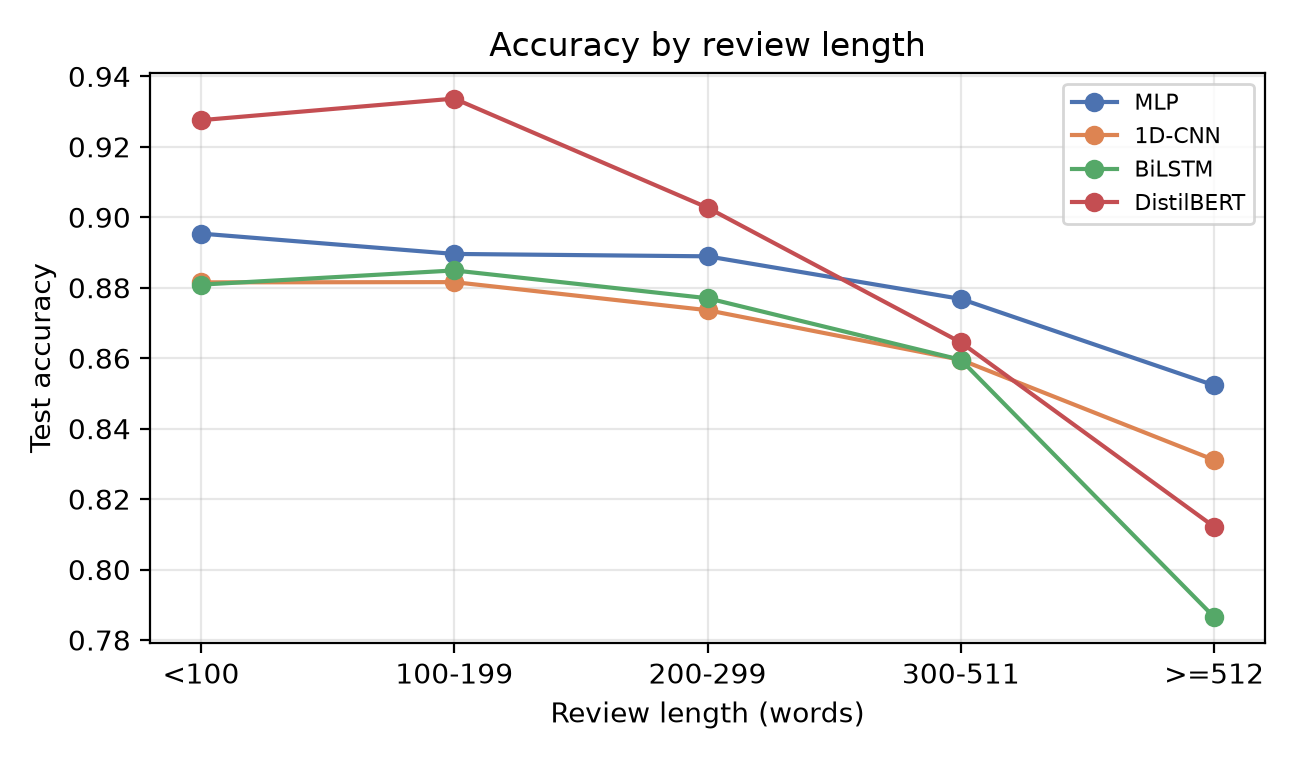
\includegraphics[width=0.66\linewidth]{accuracy_by_length.png}
\caption{Test accuracy as a function of review length in words. Bucket sizes: 3,106 / 11,747 / 4,708 / 3,645 / 1,794 reviews.}\label{fig:acclen}
\end{figure}

\begin{table}[!t]
\caption{Test accuracy (\%) on subsets of the test set}\label{tab:subsets}
\centering\footnotesize\renewcommand{\arraystretch}{1.15}
\begin{tabular}{@{}l r c c c c@{}}
\toprule
\textbf{Subset} & \textbf{Reviews} & \textbf{MLP} & \textbf{1D-CNN} & \textbf{BiLSTM} & \textbf{DistilBERT} \\
\midrule
Under 100 words      & 3,106  & 89.5 & 88.2 & 88.1 & \textbf{92.8} \\
100--199 words       & 11,747 & 89.0 & 88.2 & 88.5 & \textbf{93.4} \\
200--299 words       & 4,708  & 88.9 & 87.4 & 87.7 & \textbf{90.3} \\
300--511 words       & 3,645  & \textbf{87.7} & 86.0 & 86.0 & 86.4 \\
512 words or more    & 1,794  & \textbf{85.2} & 83.1 & 78.7 & 81.2 \\
\midrule
With a contrast word    & 19,898 & 87.9 & 86.7 & 86.3 & \textbf{90.0} \\
Without a contrast word & 5,102  & 91.2 & 89.8 & 90.6 & \textbf{94.1} \\
\bottomrule
\end{tabular}

\vspace{3pt}\parbox{0.62\linewidth}{\scriptsize Contrast words: \textit{but, however, although, though, yet, despite}.}
\end{table}

\textit{Contrast and negation.} Reviews that contain a contrast word are 3.1--4.3 points harder for every model, and the gap is largest for the BiLSTM and DistilBERT. These reviews mix praise and criticism (``the acting is fine, but the plot is absurd''), so the overall label depends on which part the reviewer weighs more. The comparison is partly confounded with length, since longer reviews are more likely to contain such words. We also measured accuracy on reviews that contain a negation word (\textit{not, no, never, n't}, \ldots), but 88\% of test reviews contain one, so that split separates almost nothing; differences on it were at most 1.6 points.

\textit{Agreement between models.} All four models are correct on 18,766 test reviews (75.1\%) and all four are wrong on 586 (2.3\%), split almost evenly between true negatives (273) and true positives (313). Table~\ref{tab:examples} shows typical cases. The reviews every model gets wrong fall into three recurring patterns: reviews that are mostly plot summary, where the opinion takes up a single sentence; mixed reviews whose positive remarks outnumber the negative ones even though the rating is low; and reviews that praise other films, so that strongly positive words refer to a different film. DistilBERT corrects 1,779 of the MLP's errors, including sarcastic reviews whose individual words look neutral or positive (Table~\ref{tab:examples}), but it also introduces 1,213 errors of its own. The two models therefore fail on noticeably different reviews, which suggests that an ensemble could outperform either one.

\begin{table}[!t]
\caption{Examples of misclassified test reviews, with each model's predicted probability of the positive class}\label{tab:examples}
\centering\footnotesize\renewcommand{\arraystretch}{1.2}
\begin{tabularx}{\linewidth}{@{}YL{1.1cm}L{4.3cm}@{}}
\toprule
\textbf{Review excerpt} & \textbf{True label} & \textbf{$P$(positive): MLP / CNN / BiLSTM / DistilBERT} \\
\midrule
``\ldots one of Hollywood's saddest swan songs \ldots It's painful to see this legendary team, the funniest duo in the history of motion pictures \ldots'' & negative & 0.85 / 0.56 / 0.71 / 0.90 \hfill (all wrong) \\
``I found the subject matter compelling, even if the conflict was a bit forced \ldots There are many continuity errors \ldots'' & negative & 0.69 / 0.95 / 0.88 / 0.95 \hfill (all wrong) \\
``\ldots Mission accomplished, Monsieur Straub. `Pretentious?' Yes. `Cinematic?' No way. This is anti-cinema.'' & negative & 0.59 / 0.39 / 0.95 / 0.04 \hfill (DistilBERT right) \\
\bottomrule
\end{tabularx}
\end{table}

%================================================================ VII
\section{Conclusion}
We compared an MLP over averaged embeddings, a 1D-CNN, a BiLSTM and a fine-tuned DistilBERT on IMDb sentiment classification under one common split, preprocessing pipeline and set of metrics. The pretrained DistilBERT is the most accurate model (90.83\% accuracy, ROC-AUC 0.970), and its advantage over every scratch model is statistically significant. Among the models trained from scratch, the order-free MLP (88.56\%) significantly outperforms both the 1D-CNN (87.32\%) and the BiLSTM (87.22\%), which are statistically tied. With only 20,000 labelled reviews and largely lexical sentiment cues, the extra capacity of the sequence models is spent on overfitting rather than on modelling word order. The error analysis showed that DistilBERT's advantage is concentrated in reviews under 300 words and reverses on very long reviews because of its 256-token input limit, and that mixed reviews containing contrast words remain the main source of error for every architecture. The choice of model is therefore a trade-off: DistilBERT gives the highest accuracy, while the MLP gives about 97\% of that accuracy at a small fraction of the computational cost.

%================================================================ VIII
\section{Future Work}
\begin{enumerate}
\item Give DistilBERT the end of long reviews, either by keeping the first and last parts of each review (the head-plus-tail truncation recommended by Sun et al.~\cite{sun2019}) or by classifying overlapping chunks and pooling the results.
\item Initialise the scratch models with pretrained GloVe vectors~\cite{pennington2014} to reduce their overfitting on 20,000 reviews.
\item Ensemble DistilBERT with the MLP, since the two models fail on different reviews.
\item Extend the comparison to fine-grained (1--10) ratings and to reviews from other domains, to test how well the conclusions generalise.
\end{enumerate}

%================================================================ BACK MATTER
\section*{Acknowledgment}
We thank the faculty of the School of Computer Engineering, MIT Manipal, for their guidance throughout this course project. We used the IMDb dataset released by Maas et al.~\cite{maas2011}, the pretrained \texttt{distilbert-base-uncased} checkpoint distributed through Hugging Face~\cite{wolf2020}, and the open-source PyTorch~\cite{paszke2019}, scikit-learn and Matplotlib libraries.

\section*{Declaration on the Use of AI Tools}
In line with the course's academic-integrity rules, we disclose that an LLM-based coding assistant (Anthropic Claude, via Claude Code) was used in Phase~3 for: (i) porting our Phase~2 Keras notebooks to the PyTorch scripts in \texttt{src/} (\texttt{data.py}, \texttt{models.py}, \texttt{train\_scratch.py}, \texttt{train\_distilbert.py}); (ii) writing the evaluation and plotting script \texttt{make\_figures.py}; and (iii) drafting the \LaTeX{} layout and an initial version of the text of this report, which the members then reviewed and rewrote. Model choices, hyperparameters and the experimental protocol come from our Phase~1 and Phase~2 work. All reported numbers are produced by running the code in the repository and were checked against the saved result files; none were written by the assistant.

\begin{thebibliography}{18}
\bibitem{maas2011}
A.~L. Maas, R.~E. Daly, P.~T. Pham, D.~Huang, A.~Y. Ng, and C.~Potts, ``Learning word vectors for sentiment analysis,'' in \emph{Proc. 49th Annu. Meeting Assoc. Comput. Linguistics (ACL)}, Portland, OR, USA, 2011, pp. 142--150.
\bibitem{kim2014}
Y.~Kim, ``Convolutional neural networks for sentence classification,'' in \emph{Proc. Conf. Empirical Methods Natural Lang. Process. (EMNLP)}, Doha, Qatar, 2014, pp. 1746--1751.
\bibitem{hochreiter1997}
S.~Hochreiter and J.~Schmidhuber, ``Long short-term memory,'' \emph{Neural Comput.}, vol.~9, no.~8, pp. 1735--1780, 1997.
\bibitem{schuster1997}
M.~Schuster and K.~K. Paliwal, ``Bidirectional recurrent neural networks,'' \emph{IEEE Trans. Signal Process.}, vol.~45, no.~11, pp. 2673--2681, Nov. 1997.
\bibitem{mikolov2013}
T.~Mikolov, I.~Sutskever, K.~Chen, G.~S. Corrado, and J.~Dean, ``Distributed representations of words and phrases and their compositionality,'' in \emph{Adv. Neural Inf. Process. Syst. (NeurIPS)}, vol.~26, 2013, pp. 3111--3119.
\bibitem{peters2018}
M.~E. Peters, M.~Neumann, M.~Iyyer, M.~Gardner, C.~Clark, K.~Lee, and L.~Zettlemoyer, ``Deep contextualized word representations,'' in \emph{Proc. NAACL-HLT}, New Orleans, LA, USA, 2018, pp. 2227--2237.
\bibitem{vaswani2017}
A.~Vaswani, N.~Shazeer, N.~Parmar, J.~Uszkoreit, L.~Jones, A.~N. Gomez, {\L}.~Kaiser, and I.~Polosukhin, ``Attention is all you need,'' in \emph{Adv. Neural Inf. Process. Syst. (NeurIPS)}, vol.~30, 2017, pp. 5998--6008.
\bibitem{devlin2019}
J.~Devlin, M.-W. Chang, K.~Lee, and K.~Toutanova, ``{BERT}: Pre-training of deep bidirectional transformers for language understanding,'' in \emph{Proc. NAACL-HLT}, Minneapolis, MN, USA, 2019, pp. 4171--4186.
\bibitem{sanh2019}
V.~Sanh, L.~Debut, J.~Chaumond, and T.~Wolf, ``{DistilBERT}, a distilled version of {BERT}: Smaller, faster, cheaper and lighter,'' in \emph{Proc. 5th Workshop Energy Efficient Mach. Learn. Cogn. Comput. (NeurIPS)}, 2019, arXiv:1910.01108.
\bibitem{howard2018}
J.~Howard and S.~Ruder, ``Universal language model fine-tuning for text classification,'' in \emph{Proc. 56th Annu. Meeting Assoc. Comput. Linguistics (ACL)}, Melbourne, Australia, 2018, pp. 328--339.
\bibitem{kingma2015}
D.~P. Kingma and J.~Ba, ``Adam: A method for stochastic optimization,'' in \emph{Proc. 3rd Int. Conf. Learn. Represent. (ICLR)}, San Diego, CA, USA, 2015.
\bibitem{srivastava2014}
N.~Srivastava, G.~Hinton, A.~Krizhevsky, I.~Sutskever, and R.~Salakhutdinov, ``Dropout: A simple way to prevent neural networks from overfitting,'' \emph{J. Mach. Learn. Res.}, vol.~15, no.~56, pp. 1929--1958, 2014.
\bibitem{loshchilov2019}
I.~Loshchilov and F.~Hutter, ``Decoupled weight decay regularization,'' in \emph{Proc. 7th Int. Conf. Learn. Represent. (ICLR)}, New Orleans, LA, USA, 2019.
\bibitem{sun2019}
C.~Sun, X.~Qiu, Y.~Xu, and X.~Huang, ``How to fine-tune {BERT} for text classification?,'' in \emph{Proc. China Nat. Conf. Chinese Comput. Linguistics (CCL)}, Kunming, China, 2019, pp. 194--206.
\bibitem{zhang2017}
Y.~Zhang and B.~Wallace, ``A sensitivity analysis of (and practitioners' guide to) convolutional neural networks for sentence classification,'' in \emph{Proc. 8th Int. Joint Conf. Natural Lang. Process. (IJCNLP)}, Taipei, Taiwan, 2017, pp. 253--263.
\bibitem{wolf2020}
T.~Wolf \emph{et~al.}, ``Transformers: State-of-the-art natural language processing,'' in \emph{Proc. Conf. Empirical Methods Natural Lang. Process.: System Demonstrations (EMNLP)}, 2020, pp. 38--45.
\bibitem{paszke2019}
A.~Paszke \emph{et~al.}, ``{PyTorch}: An imperative style, high-performance deep learning library,'' in \emph{Adv. Neural Inf. Process. Syst. (NeurIPS)}, vol.~32, 2019, pp. 8024--8035.
\bibitem{pennington2014}
J.~Pennington, R.~Socher, and C.~D. Manning, ``{GloVe}: Global vectors for word representation,'' in \emph{Proc. Conf. Empirical Methods Natural Lang. Process. (EMNLP)}, Doha, Qatar, 2014, pp. 1532--1543.
\end{thebibliography}

%================================================================ C.3
\clearpage
\section*{C.3: Individual Contribution Statement}
Each member owned one model: its design and hyperparameters, its training and evaluation, and its subsection of Section~IV, and each member presents that model at the final presentation. Shared work is listed against the member who did it.

\vspace{4mm}
\begin{table}[!h]
\centering\footnotesize\renewcommand{\arraystretch}{1.3}
\begin{tabularx}{\linewidth}{@{}L{2.6cm}L{1.6cm}L{2.4cm}YL{2.5cm}@{}}
\toprule
\textbf{Member Name} & \textbf{Reg. No.} & \textbf{Model / Task Owned} & \textbf{Key Contributions} & \textbf{Signature}\\
\midrule
Harshavardhan Reddy & 230953396 & BiLSTM; shared pipeline, experiments and integration & Designed and trained the BiLSTM (packed sequences, spatial and input dropout, reduced learning rate) and wrote its analysis. Created and maintained the team GitHub repository and its README automation. Wrote the shared data pipeline (common stratified split, train-only tokenizer, evaluation and result-saving code) used by all four models. Ran the final training and test evaluation of all four models on a local GPU. Produced the comparison table, figures, McNemar tests and error analysis, and assembled the final report and presentation. & \raisebox{-0.85\height}{\includegraphics[width=2.4cm,height=9mm,keepaspectratio]{signatures/sig_harsha.png}}\\
\midrule
Meesha Gupta & 230953090 & DistilBERT & Selected DistilBERT and its fine-tuning settings (AdamW, warm-up and decay, learning rate, 256-token input limit, early stopping); reviewed the attention and transfer-learning literature; wrote the DistilBERT subsection and analysed its results, including its weakness on long reviews. & \raisebox{-0.85\height}{\includegraphics[width=2.4cm,height=9mm,keepaspectratio]{signatures/sig_meesha.png}}\\
\midrule
Ratul Jha & 230953338 & 1D-CNN & Built the multi-width (3, 4, 5) 1D-CNN and chose its filter, dropout, batch-size and early-stopping settings; reviewed the convolutional text-classification literature; wrote the 1D-CNN subsection and analysed its results, including its bias towards the positive class. & \raisebox{-0.85\height}{\includegraphics[width=2.4cm,height=9mm,keepaspectratio]{signatures/sig_ratul.png}}\\
\midrule
Kshitij Singh & 230953460 & MLP & Built the MLP baseline over masked mean-pooled embeddings and chose its dropout and regularisation settings; reviewed the word-representation literature; wrote the MLP subsection and analysed why the baseline outperforms the sequence models. & \raisebox{-0.85\height}{\includegraphics[width=2.4cm,height=9mm,keepaspectratio]{signatures/sig_kshitij.png}}\\
\bottomrule
\end{tabularx}
\end{table}

\vspace{6mm}
\noindent We confirm that the contributions listed above are accurate, and each of us is prepared to be questioned individually on the work stated against our name.

\end{document}
